\subsection{Experiments with least latency adaptation}
\label{sec:leastlatency}
%Internet users often leverage location diversity by downloading a file from the closest location it is available. 
%For example, CDNs direct users to the least latency server location, and users choose nearby  mirror sites for file download.


In experiments until now, users leverage location diversity by downloading a file in parallel from all locations. Next, we present our experiment with least latency adaptation in which a user downloads a file from the closest location it is available. 
This adaptation is inspired by redirection schemes that are widely used by CDNs today \cite{Akamai2002,donar}.
These experiments reinforce our earlier finding that all TE schemes achieve nearly the same SPF values when applications adapt to location diversity.
With least latency adaptation, an increase in location diversity yields little improvement in SPF of any TE scheme.
This adaptation reduces the SPF of \opt\ to bridge the gap between \opt\ and sub-optimal schemes such as \optwt.




\eat
{
Real-world systems especially CDNs \cite{Akamai2002,donar} use various forms of this adaptation account for  server load, datacenter bandwidth, round trip delay, network loss rates, billing costs at each server deployment, and so on \cite{Akamai2002,donar}.


In experiments in Section \ref{sec:capacity}, users leverage location diversity by downloading a file in parallel from all locations.
Another common approach to leverage location diversity is to download a file from the closest location it is available.
Real-world systems use various forms of this adaptation, which we call \emph{least latency adaptation}. 
These adaptations account for  server load, datacenter bandwidth, round trip delay, network loss rates, billing costs at each server deployment, and so on \cite{Akamai2002,donar}.


Accurately modeling all these factors is a complex problem, and is beyond the scope of this work.
}

%In Section \ref{sec:capacity}, users download a file from all locations the file is available using parallel TCP connections.
%In this section, we experiment with another common approach to leverage location diversity - 
%a user downloads a file from the closest location it is available. 
%In general, real-world systems use various forms of \emph{least latency adaptation} accounting for  server load, datacenter bandwidth, round trip latency, network loss rates, billing costs at each server deployments, and so on \cite{Akamai2002,donar}.
%Accurately modeling all these factors is a complex problem, and is beyond the scope of this work.


%In the previous section, users downloaded a file from all locations the file is available using parallel TCP connections. 
%In this section, we experiment with another common approach to leverage location diversity - 
%a user downloads a file from the closest location it is available. 
%The distance between the user and the file location is measured as the propagation delay along the path between them.
%If there are multiple paths between two locations, we measure propagation delay as the weighted average of latencies of all paths; 
%the weight of a path is equal to the fraction of traffic it carries from source to the destination node.  
%This adaptation is called the least latency adaptation.

%However, least latency adaptation that we consider does not depend on the congestion in the network, i.e., the user chooses the same (closest) replica irrespective of the congestion on the path from that replica to the user.

%We seek to answer two main questions through our experiments with least latency adaptation.  
%As before, we vary the location diversity for each file keeping the total traffic requested by each node unchanged.
%First, we ask whether the effective capacity of the network to tolerate surges in traffic demand increases with location diversity.
%Second, we compare the relative performance of TE schemes accounting for location diversity.  
%We use SPF metric to compare TE schemes.


%We use  flow-level simulations instead of  packet level simulations for this set of experiments. Flow-level simulations are two  orders of magnitude faster than packet level simulations (few hundred seconds vs. few hours).  Moreover, flow-level simulations suffice to measure the  traffic between any two PoPs in this experiment. In comparison, our earlier experiments with parallel downloads required packet-level simulations to measure PoP-to-PoP traffic. This difference arises because least latency adaptation allows a user to download each file from one location only but a user downloads a fraction of a file from every location in case of  parallel downloads. In the latter case,  these fractions can only be estimated if the TCP throughputs of all connections are known; accurate estimation of TCP throughputs requires packet-level simulations. WIth least latency adaptation, flow-level simulations calculate the sum of sizes of files downloaded  at a PoP from any other PoP.

\subsubsection{Experiment procedure}


We model least latency adaptation as follows: a user downloads a file from the location that has the smallest propagation delay.
If there are multiple paths between two locations, propagation delay is measured as the weighted average of latencies of all paths; 
the weight of a path is equal to the fraction of traffic it carries.
To emulate a location diversity of $k$, each file is replicated at the original location based on traffic matrix and at $(k-1)$ additional locations. 
We select additional locations such that the probability of replicating a file at a location is proportional to its total outgoing link capacity. 
%Which location a user downloads a file from depends on two factors. 
%First, on the set of locations at which a file is available. 
%Second, on the routing in the network, which affects the propagation delay of paths. 


%Each file is replicated at the original location based on traffic matrix and at $(k-1)$ additional locations.  We select additional replica locations of a file such that the probability of placing a replica at a location is proportional to its total outgoing link capacity. 

%\subsubsection{Flow-level simulations}

We use  flow-level simulations instead of  packet level simulations for this set of experiments. 
Flow-level simulations are two  orders of magnitude faster than packet-level simulations (few hundred seconds vs. few hours).  
Moreover, flow-level simulations suffice to measure SPF in this experiment. 
Our earlier experiments with parallel downloads require packet-level simulations to measure PoP-to-PoP traffic, and hence SPF.
In case of  parallel downloads, a user downloads fractions of a file from multiple locations.
The fractions of a file downloaded from all locations can only be estimated if TCP throughput of every connection is known. 
We use packet-level simulations to accurately estimate TCP throughput in the earlier experiment.

%To accurately estimate TCP throughput of every connection, we use packet-level simulations.


%In this experiment, flow-level simulations calculate PoP-to-PoP traffic as follows.
%The incoming traffic rate at a PoP from any other PoP,  is calculated as the sum of sizes of files requested at this PoP from another PoP divided by the experiment duration.
%
%
%As before, we compute SPF for multiple levels of location diversity (k = 1, 3, 5 and 7). 
%We select additional replica locations of a file such that the probability of placing a replica at a location is proportional to its total outgoing link capacity. 



%SPF computation is straight forward once link utilizations are computed. 
%We increase the surge factor  for a TM in small increments as before and measure the MLU at every step. 
%The surge factor at which the MLU exceeds one is the SPF. 


%Multiplying the fraction of flows between the PoPs that cross a link by the PoP-to-PoP traffic, gives 
%Next, we calculate the fraction of this traffic that crosses a link, which is equal to the fraction of flows between the PoPs that cross the link.
%Given the traffic between two PoPs, we calculate the traffic on each link as the fraction of flows between the PoPs that cross this link.
%The total traffic on a link is calculated as the sum of PoP-to-PoP traffic that crosses this link for all pairs of PoPs. 


%Our flow-level simulations calculate PoP-to-PoP traffic by the sum of sizes of files requested at the destination PoP from the source PoP divided by the experiment duration.
%The incoming traffic rate at a PoP from any other PoP,  is calculated as the sum of sizes of files requested at this PoP from another PoP divided by the experiment duration.

To calculate SPF, flow level simulations measure PoP-to-PoP traffic and link utilizations.
PoP-to-PoP traffic (in bits/sec) is equal the sum of sizes of files requested at the sink PoP from another PoP divided by the experiment duration.
For a pair of PoPs, the PoP-to-PoP traffic crossing a link is equal to the fraction of flows between the PoPs that cross this link times the PoP-to-PoP traffic.
Summing the PoP-to-PoP traffic that crosses a link for all pairs of PoPs gives the total traffic on a link, which yields link utilization.
We increase the surge factor  for a TM in small increments as before. The least surge factor at which any link utilization exceeds 1 is the SPF.

%
%incoming traffic rate at a PoP from any other PoP  is calculated as the sum of sizes of files requested at this PoP from another PoP divided by the experiment duration.
%For a pair of PoPs, the PoP-to-PoP traffic crossing a link is equal to the fraction of flows between the PoPs that cross this link times the PoP-to-PoP traffic.
%Summing the PoP-to-PoP traffic that crosses a link for all pairs of PoPs gives the total traffic on a link, which yields link utilization.


%SPF computation is straight forward once link utilizations are computed. 
%We increase the surge factor  for a TM in small increments as before. The least surge factor at which traffic on a link exceeds capacity is the SPF.
%We compute SPF for multiple levels of location diversity (k = 1, 3, 5 and 7). 
%We select additional replica locations of a file such that the probability of placing a replica at a location is proportional to its total outgoing link capacity. 

\eat{
SPF computation is straight forward once link utilizations are computed. 
We increase the surge factor  for a TM in small increments as before and measure the MLU at every step. 
The surge factor at which the MLU exceeds one is the SPF. 
We compute SPF for multiple levels of location diversity (k = 1, 3, 5 and 7). 
We select additional replica locations of a file such that the probability of placing a replica at a location is proportional to its total outgoing link capacity. 
}

%As before, we vary the location diversity for each file keeping the total traffic requested by each node unchanged. We select additional replica locations such that the probability of placing a replica at a node is proportional to its total outgoing link capacity. 

%The locations of the replicas of a file influences traffic demand patterns, which affects the SPF metric. We experiment with two replica selection strategies. First, we place replicas at randomly selected nodes. Second, we place replicas such that the probability of placing the replica at a node is proportional to the sum of its outgoing links capacities. In both cases, no two replicas are placed at the same node. TBD: Do we need this.



\begin{figure}[t] 
\begin{center} 
\subfigure{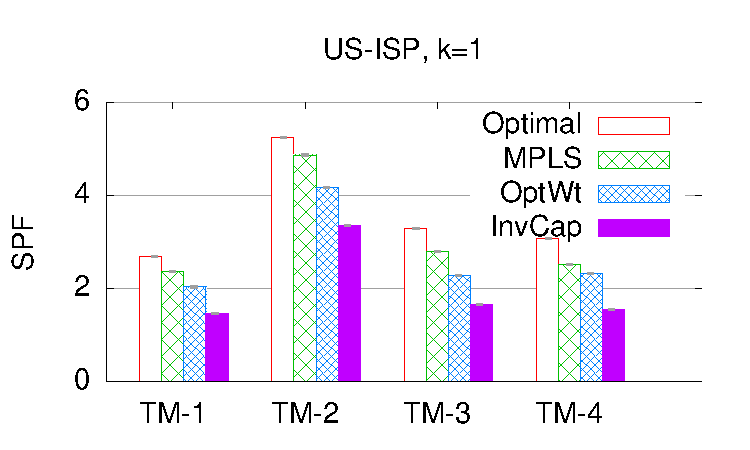
\includegraphics[scale=0.5]{newimages/ATT2/k1_MLU.pdf}}
\subfigure{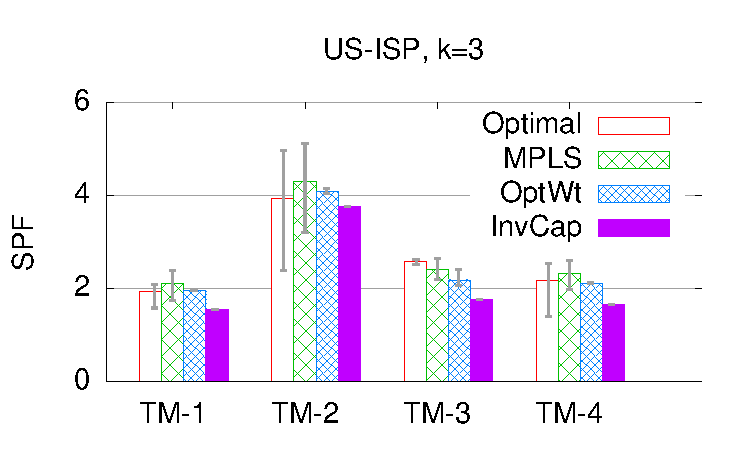
\includegraphics[scale=0.5]{newimages/ATT2/k3_MLU.pdf}}
\subfigure{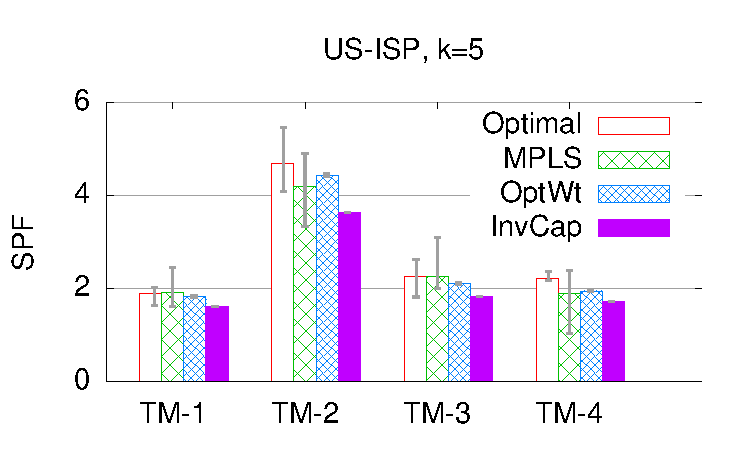
\includegraphics[scale=0.5]{newimages/ATT2/k5_MLU.pdf}}
\subfigure{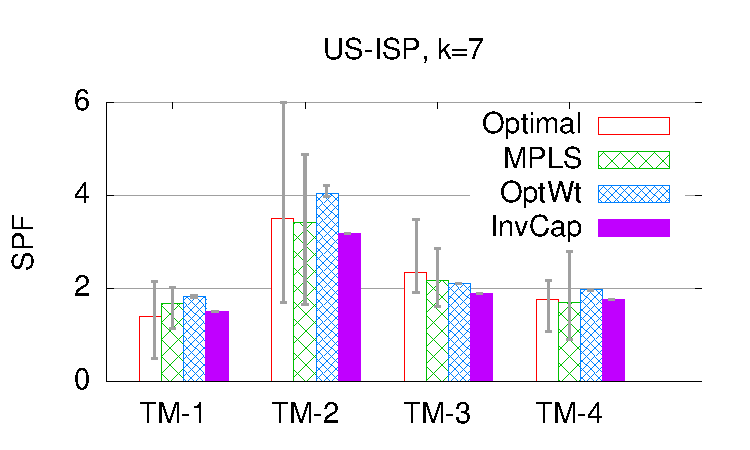
\includegraphics[scale=0.5]{newimages/ATT2/k7_MLU.pdf}}
 \end{center}
 \vspace{-0.2in}
\caption{[US-ISP] Mean SPF values of TE schemes with least latency adaptation. Error bars show the maximum and minimum SPF values over 20 repetitions. At higher location diversity, SPF values do not increase, in some cases even reduce, as location diversity increases from k = 1 to k = 7.}
\vspace{-0.2in}
\label{fig:leastlatspf}
\end{figure}


\begin{figure}[t] 
\begin{center}
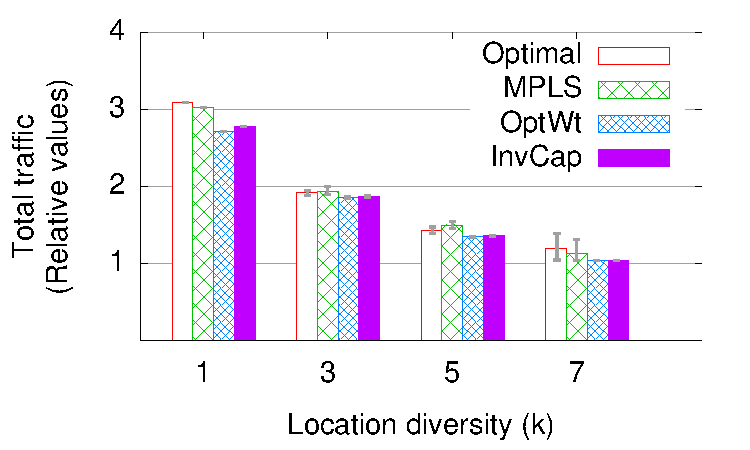
\includegraphics[scale=0.5]{newimages/ATT2/TM27_totalTraffic.pdf}
\end{center}
\vspace{-0.2in}
\caption{[US-ISP, Traffic matrix TM-1, surge factor = 1]  Due to least latency adaptation, total traffic reduces to one-third as location diversity increases from k = 1 to k = 7.  Despite reduction in total traffic, SPF does not improve.}
\vspace{-0.2in}
\label{fig:totaltraffic}
\end{figure}



\subsubsection{Results}


We discuss here the results for the Tier-1 US ISP network. 
The Abilene and Geant topologies show qualitatively similar conclusions.
Figure \ref{fig:leastlatspf} shows the SPF values for four traffic matrices (same TMs as in Figure \ref{fig:capacity_diversity}). 
Location diversity increases from the top  graph (k = 1)  to the bottom graph (k = 7).
In a network with location diversity  (k = 3, 5, 7), all schemes including \opt\ have nearly same SPF values.
In comparison, \opt\ has higher SPF than other schemes in the absence of location diversity (k = 1). 
Even a static routing scheme, \invcap\ is at most 20\% worse compared to \opt.
In our experiments with the Abilene and Geant topologies, \invcap\ is at most 30\% worse compared to \opt. 
These observations are consistent with our findings in earlier set of experiments with parallel downloads.



%\opt\ has higher SPF than other schemes in the absence of location diversity (Figure 14, k = 1).
%In a network with location diversity  (k = 3, 5, 7), all schemes including \opt\ have nearly same SPF values. 
%Even a static routing scheme, \invcap\ is at most 20\% worse compared to \opt.
%In our experiments with the Abilene and Geant topologies, \invcap\ is at most 30\% worse compared to \opt. 
%In Section \ref{sec:capacity}, we found that application adaptation to location diversity reduces the difference between ``no TE'', i.e., \invcap\ and schemes that engineer traffic such as \opt. 
%Further, which TE scheme is used makes little difference to SPF.
%Our experiments with least latency adaptation reinforces both these findings.

Contrary to expectation, increasing location diversity yields little improvement in SPF of any TE scheme.
In Figure \ref{fig:leastlatspf}, the bars for each TM in the top graph (k = 1) are nearly as  tall as the bars in the bottom graph (k = 7). 
In some cases, bars in the bottom graph are slightly shorter, that is, SPF worsens on increasing location diversity, e.g.,  TM-2 for \opt.


With more location diversity, the utilization  of most links reduces dramatically.
This is evident from Figure 15, which shows the total traffic on all links at different levels of location diversity for a US-ISP  traffic matrix.
The total traffic on all links at k = 7 is one-third of the total traffic at k = 1 for every scheme.
But the peak link utilization does not reduce, it even increases in some cases, as location diversity increases.
This is why SPF does not improve despite a reduction in total traffic. 

Contrary to expectation, SPF yields no improvement with increasing location diversity.
In Figure \ref{fig:leastlatspf}, the bars for each TM in the top graph (k = 1) are nearly as  tall as the bars in the bottom graph (k = 7). 
In some cases, bars in the bottom graph are slightly shorter, that is, SPF worsens on increasing location diversity, e.g.,  TM-2 for \opt.


Figure 15 shows the total traffic on all links at different levels of location diversity for a US-ISP  traffic matrix. In this graph, the surge factor is always equal to 1, so the aggregate demand at end-nodes remains the same. But, the total traffic on all links at k = 7 is one-third of the total traffic at k = 1 for every scheme.

%For a single traffic matrix (TM-1), Figure \ref{fig:totaltraffic} shows the total traffic on all links for all location diversity levels. 

%On the other hand, the total traffic on all links  reduces to one-third for all TE schemes as location diversity increases from k = 1 to k = 7 (Figure \ref{fig:totaltraffic}). 
With more location diversity, users, on average, download files from a location closer than before.
This reduces the total traffic on all links, and reduces utilization of most links.
But the maximum link utilization does not reduce, it even increases in some cases, as location diversity increases. 
The most utilized link is the first to experience congestion at higher surge factors.
Least latency adaptation does not respond to congestion by moving traffic from the most utilized link to other under-utilized links.
It always downloads from the least propagation delay location, irrespective of the congestion on the path from that location.
This is why SPF does not improve despite a reduction in total traffic. 
An implication of this finding is that an adaptation scheme must be responsive to network congestion to leverage location diversity and increase the network's tolerance to traffic demand surges.



%Figure 15 shows a different metric: the total traffic on all links at different levels of location diversity for a US-ISP  traffic matrix.
%In this graph, the surge factor is always equal to 1, so the aggregate demand at end-nodes remains the same. 
%But, the total traffic on all links at k = 7 is one-third of the total traffic at k = 1 for every scheme.

%Figure 15 shows the total traffic on all links at different levels of location diversity for a US-ISP  traffic matrix. 
%In this graph, the surge factor is always equal to 1, so the aggregate demand at end-nodes remains the same. 
%But, the total traffic on all links at k = 7 is one-third of the total traffic at k = 1 for every scheme.

%For a single traffic matrix (TM-1), Figure \ref{fig:totaltraffic} shows the total traffic on all links for all location diversity levels. 

%On the other hand, the total traffic on all links  reduces to one-third for all TE schemes as location diversity increases from k = 1 to k = 7 (Figure \ref{fig:totaltraffic}). 
%With more location diversity, users, on average, download files from a location closer than before. 
%This is evident from Figure 15, which shows the total traffic on all links at different levels of location diversity for a US-ISP  traffic matrix.
%The total traffic on all links at k = 7 is one-third of the total traffic at k = 1 for every scheme.
%Increase in location diversity reduces utilization of most links.
%But the maximum link utilization does not reduce, it even increases in some cases, as location diversity increases. 
%The most utilized link is the first to experience congestion at higher surge factors.

Least latency adaptation does not respond to congestion by moving traffic from the most utilized link to other under-utilized links.
It always downloads from the least propagation delay location, irrespective of the congestion on the path from that location.
An implication of this finding is that an adaptation scheme must be responsive to network congestion to leverage location diversity and increase the network's tolerance to traffic demand surges.

%Location diversity blurs differences between TE schemes.





\eat{

We discuss here the results for the Tier-1 US ISP network. 
The Abilene and Geant topologies show qualitatively similar conclusions.
Figure \ref{fig:leastlatspf} shows the SPF values for four traffic matrices (same TMs as in Figure \ref{fig:capacity_diversity}). 
Location diversity increases from the top  graph (k = 1)  to the bottom graph (k = 7).
Contrary to expectation, SPF yields no improvement with increasing location diversity.
In Figure \ref{fig:leastlatspf}, the bars for each TM in the top graph (k = 1) are nearly as  tall as the bars in the bottom graph (k = 7). 
In some cases, bars in the bottom graph are slightly shorter, that is, SPF worsens on increasing location diversity, e.g.,  TM-2 for \opt. 
Figure 15 shows the total traffic on all links at different levels of location diversity for a US-ISP  traffic matrix. In this graph, the surge factor is always equal to 1, so the aggregate demand at end-nodes remains the same. But, the total traffic on all links at k = 7 is one-third of the total traffic at k = 1 for every scheme.

%For a single traffic matrix (TM-1), Figure \ref{fig:totaltraffic} shows the total traffic on all links for all location diversity levels. 

%On the other hand, the total traffic on all links  reduces to one-third for all TE schemes as location diversity increases from k = 1 to k = 7 (Figure \ref{fig:totaltraffic}). 
With more location diversity, users, on average, download files from a location closer than before.
This reduces the total traffic on all links, and reduces utilization of most links.
But the maximum link utilization does not reduce, it even increases in some cases, as location diversity increases. 
The most utilized link is the first to experience congestion at higher surge factors.
Least latency adaptation does not respond to congestion by moving traffic from the most utilized link to other under-utilized links.
It always downloads from the least propagation delay location, irrespective of the congestion on the path from that location.
This is why SPF does not improve despite a reduction in total traffic. 
An implication of this finding is that an adaptation scheme must be responsive to network congestion to leverage location diversity and increase the network's tolerance to traffic demand surges.

%Location diversity blurs differences between TE schemes.


\opt\ has higher SPF than other schemes in the absence of location diversity (Figure 14, k = 1).
In a network with location diversity  (k = 3, 5, 7), all schemes including \opt\ have nearly same SPF values. 
Even a static routing scheme, \invcap\ is at most 20\% worse compared to \opt.
In our experiments with the Abilene and Geant topologies, \invcap\ is at most 30\% worse compared to \opt. 
In Section \ref{sec:capacity}, we found that application adaptation to location diversity reduces the difference between ``no TE'', i.e., \invcap\ and schemes that engineer traffic such as \opt. 
Further, which TE scheme is used makes little difference to SPF.
Our experiments with least latency adaptation reinforces both these findings.

}


%TBD: Why variances so high?
%TBD: In another experiment, we place replicas at randomly selected nodes. However our results remain unchanged.

%Our experiments with least latency adaptation reinforce our earlier finding that application adaptation to location diversity reduces the difference between ``no TE'', i.e., \invcap\ and schemes that engineer traffic such as \opt.  
%Further, which TE scheme is used makes little difference to SPF.

%These experiment also show the SPF may not improve even with a higher location diversity unless the adaptation scheme is responsive to network congestion, e.g. the adaptation scheme of parallel TCP downloads,  to 


%TBD: Why variances so high?
%
%TBD: Conclusions here.
